%----------------------------------------------------------------------------
\chapter{A feladat} \label{sec:feladat}
%----------------------------------------------------------------------------
	A minta egy fémezett felület, aminek magasságtérképét mérések eredményeként 
	adott pontossággal ismerjük.
	A magasságmérések egy négyzetes háló felett történtek, amelynek mindkét irányában
	$\delta_x = \delta_y \simeq 120 nm$ azonos a felbontása
	A magasságmérés függőleges pontossága $\delta_z \simeq 20nm$ volt.
	A töltéssűrűség méréséhez szükséges második pásztázás során a tűt a mintához képest $V_{tu} = 500 mV$ potenciálra kapcsoljuk.
	Illetve a fémezett felülettől közel azonos távolságra rezegtetjük és a (hosszú hegyes) tűre ható erőt mérjük.
	
	\noindent A dolgozatban felhasznált magasságtérkép-mérési eredmény (\ref{fig:felulet}. ábra) egy
	$512\times512$ méretű szürkeárnyalatos *.tiff állomány, amely értéke $0-255$-ig terjed.
	A mérőberendezés adatlapja alapján és a mérés végén megjelenített konstansokkal lehetséges a kép skálázása.
	
	\begin{figure}[!h]
		\centering
		\subfloat[Mérési eredmény]{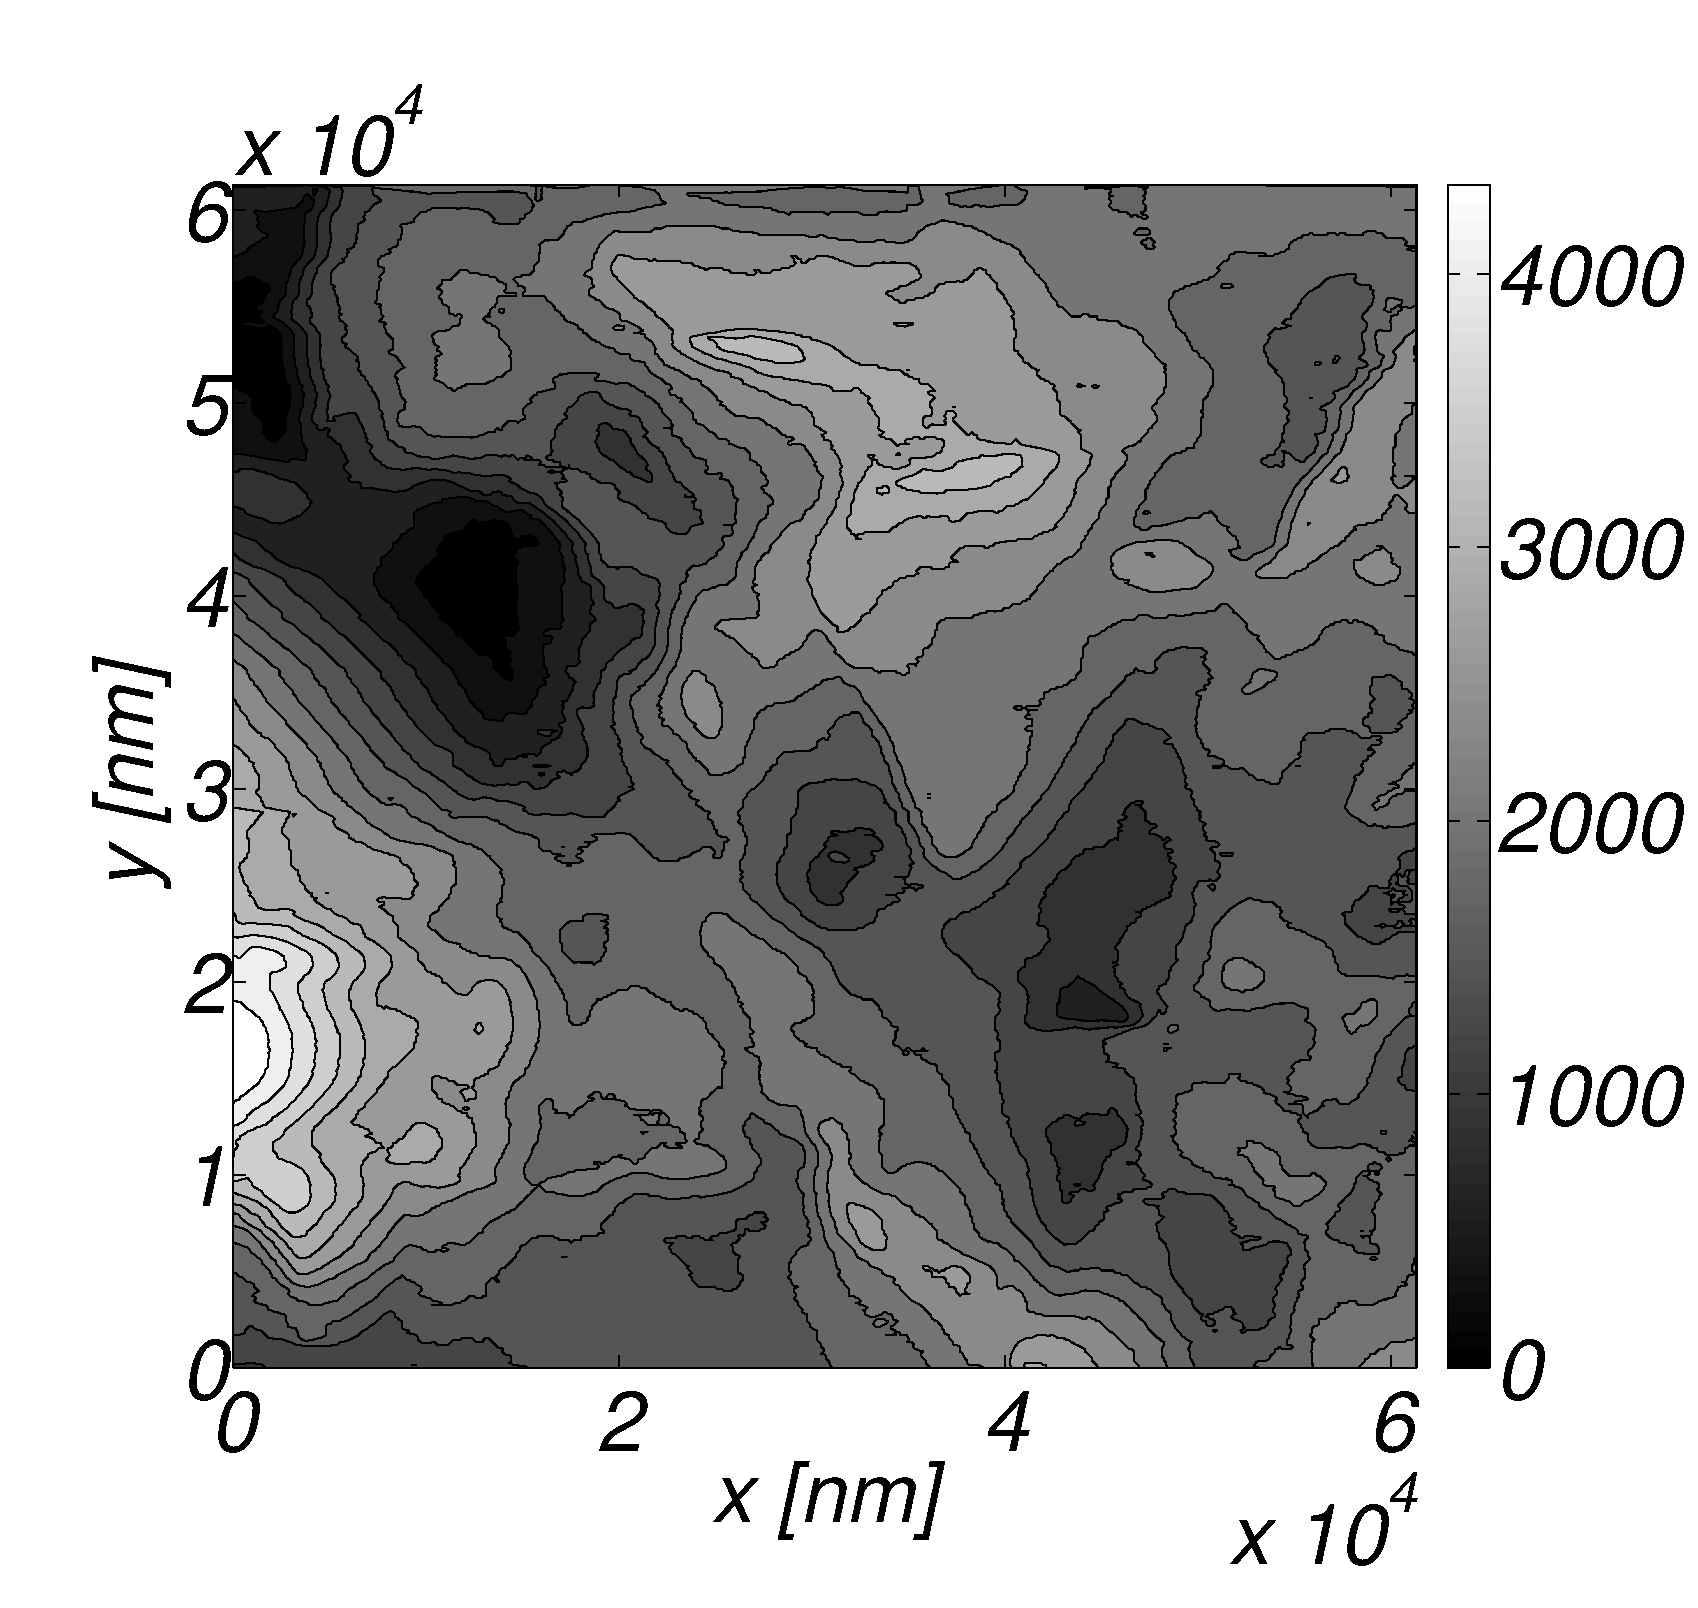
\includegraphics[width=0.6\columnwidth]{figures/eps/newafm_total.eps}%
		\label{fig:afm_total}}
		\hfil
		\subfloat[Mérés részlete]{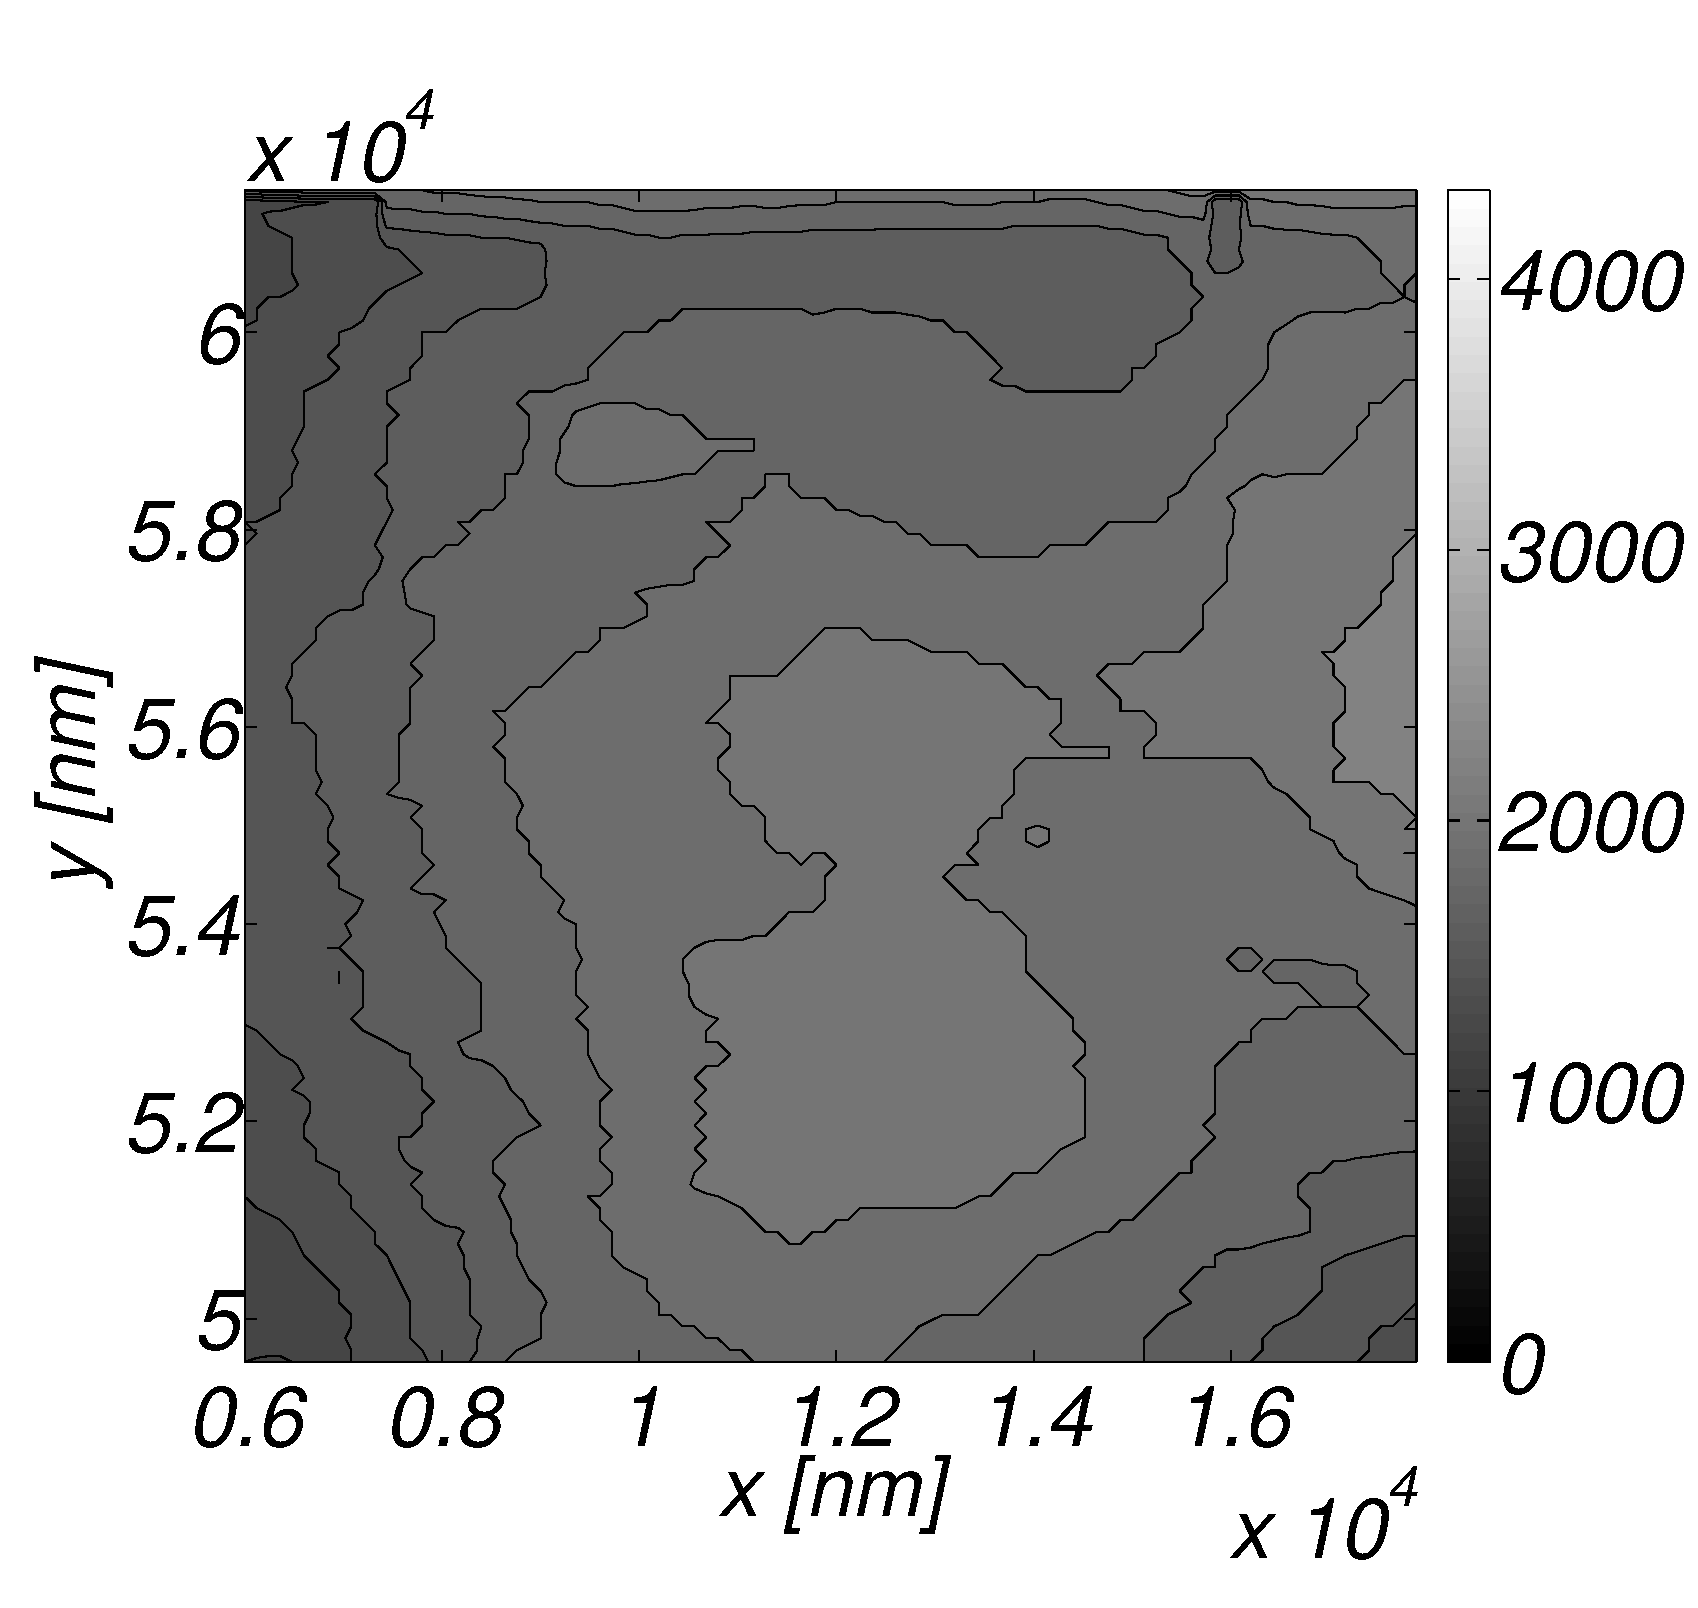
\includegraphics[width=0.3\columnwidth]{figures/eps/newafm200.eps}%
		\label{fig:afm200}}
		\caption{Méréssel kapott magasságtérkép. Felbontás $d_x=d_y=120nm \ d_z=18.03nm$}
		\label{fig:felulet}
	\end{figure}
	
	\noindent
	A dolgozat céljául egy olyan szimulátor építését tűztem ki, amely segítségével közel valós időben 
	lehetséges a mérés alapján a felületi töltéseloszlásról a mérőeszköz pontosságánál finomabb felbontást elérni.
	
	
	
\section{Fizikai probléma matematikai formalizálása}
	
	A megoldandó feladat egy elektrosztatikus feladat.
	A minta és a tű közötti térben nincsenek töltések, így itt a Poisson egyenlet helyett a
	Laplace-egyenlet \ref{eq:laplace} érvényes.
	\begin{equation}\label{eq:laplace}
		\Delta V(x,y,z) = 0 
	\end{equation}
	Az egyenletet a következő részben (\ref{sec:sim_terfogat}) ismertetett  megfontolások végett egy redukált
	3D-s térfogatban oldom meg.
	Ezen 3D-s térfogatra egy inhomogén ponthálót illesztünk, amelynek vízszintesen $d_{ax} = d_{ay}$,
	függőlegesen $d_z$ a felbontása, ami a használt AFM apparátus felbontásával $d_z = \delta_z$ egyezik meg.
	Az így kapott térbeli háló minden pontjához hozzárendeljük az $V_{i,j,k} \simeq V(id_x,jd_y,kd_z)$
	potenciált.
	Dirichlet határfeltételek a felület fémezése, amely zérus potenciálú és az adott ($V_{tu} = 500mV$)
	potenciálú  tű fémes felülete.
	A térnek a minta és a tű felületétől különböző határfelületén homogén Neumann feltételt alkalmazunk
	az elhanyagolások (végtelen tér) és a töltésmentesség miatt.
	
	Az így adódó lineáris egyenletrendszer megoldására lehetséges direkt és iteratív megoldó
	algoritmusokat alkalmazni.
	%($1\leq i\leq i_{max}$, $1\leq j\leq j_{max}$, $1\leq k\leq k_{max}$). 
% 	Az alkalmazott interpoláció során a függőleges irányú felbontást is figyelembe véve
	\begin{changebar}
	A párhuzamosítási szándékok miatt az iteratív megoldást választottuk, mivel a multiprocesszoros
	környezetek tipikusan kevés fajlagos-memóriával
	\footnote{Fajlagos alatt az egy szimulációra jutó
	memóriát értem. (Természetesen ezen szimulációk egyszerre futnak, így a fajlagos-memória
	akkumulálódik.)} rendelkeznek.
	\end{changebar}
	%\todo[prepend]{lokál-t én basztatom és a cache lelassít ekkor a BANK conflict 	miatt}
	Ekkor nem teljesen pontos megoldást kapunk, azonban gyorsabban juthatunk el az elfogadható eredményhez.
	A számítási pontosság növelhető az iterációt leállító konvergencia követelmény keményebb
	megszabásával, ami persze több iterációt jelent.
	
	Az iteratív megoldás során a megoldás aktuális értékének kiszámításához az előző megoldásból indulunk ki.
	A \eqref{eq:laplace} egyenletben szereplő deriválást az elsőrendű Taylor közelítés alkalmazásával a
	\eqref{eq:it} szerinti 6-pontos sémát kapjuk.
	\begin{equation} \label{eq:it} 
		V_{ijk}^{n+1} = \\ \Delta_1 \cdot \left(V_{i-1,j,k}^n+V_{i+1,j,k}^n
		+V_{i,j-1,k}^n+V_{i,j+1,k}^n\right)+ \\
						\Delta_2 \cdot \left(V_{i,j,k-1}^n+V_{i,j,k+1}^n\right)
	\end{equation}
	ahol $V_{i,j,k}^n$ az az $n$-dik iterációs lépésben az $i,j,k$ indexű
	pontban mérhető potenciált jelöli, $\Delta_1$ a vízszintes felbontásból,
	$\Delta_2$ a függőleges felbontásból adódó állandó.
	%Az iterációs eljárás előnye, hogy implementációja egyszerűbb és a
	%\eqref{eq:2} szerinti ``simítás'' gyorsabb, mint a direkt megoldás.
	%Az iterációs eljárás előnye, hogy memóriaigénye kicsi a direkt megoldás során
	% adódó egyenletmegoldáshoz képest.
	%Hátránya hogy nem ad pontos választ egy lépésben.
	
% 	\begin{figure}[!ht]
% 		\centering
% 		\psfrag{ijk}{$(i,j,k)$}
% 		\psfrag{imjk}{$(i-1,j,k)$} 
% 		\psfrag{ipjk}{$(i+1,j,k)$}
% 		\psfrag{ijmk}{$(i,j-1,k)$} 
% 		\psfrag{ijpk}{$(i,j+1,k)$}
% 		\psfrag{d1}{$k_x$} 
% 		\psfrag{d2}{$k_y$} 
% 		\psfrag{d3}{$k_z$} 
% 		\psfrag{ijkm}{$(i,j,k-1)$} 
% 		\psfrag{ijkp}{$(i,j,k+1)$} 
% 		\includegraphics[width=0.95\columnwidth]{kepek/eps/sema.eps}
% 		\caption{\scriptsize Diszkretizálás során alkalmazott felosztás} 
% 	\end{figure}

	
% 	fi(idx,idy,idz) = KK1*(fip(idx-1,idy,idz)+fip(idx+1,idy,idz)+fip(idx,idy-1,idz)+fip(idx,idy+1,idz))+...
%               KK2*(fip(idx,idy,idz-1)+fip(idx,idy,idz+1))

\section{Szimulálandó térfogat} \label{sec:sim_terfogat}
\subsection{Szimulálandó térfogat alapja}
	A felületmérés során a minta-tű távolsága jóval kissebb a mérési pontok vízszintes távolságánál (lásd \ref{fig:afm}. ábra).
	\begin{equation}
	D=[5,50]\ nm\quad \ll \quad \delta_x=\delta_y=120nm 
	\end{equation}
	A Coulomb-kölcsönhatás a távolság négyzetével fordítottan arányos, így az előbb említettek értelmében egy mérési pont néhány 
	szomszédjáig, pontosabban a mérési pont egy redukált környezetét szükséges csupán szimulálni.
	Hiszen azon kívül már elhanyagolható a villamos térerősség.
	(Másképpen megfogalmazva a vízszintes mérési pontok távolsága jóval nagyobb mint a Coulomb-kölcsönhatás effektív távolsága).
	
	A tipikus AFM tűk terét a MATLAB Partial Differential Equiation Toolbox-al szimuláltam.
	A szimulációt $1000\times 1000\times 1000\ nm$-es térfogaton $\sim5000$ elemmel végeztem, a tű $V_{tu} = 500mV$ potenciálja
	esetén.
	\begin{itemize}
	  \item A minta-tű távolság: $D=20\ nm$,
	  \item tű sugara $R=5\ nm$,
	  \item kúp fél nyílásszöge hegyes A típusú $Si$ esetén $\Theta=10\degree$,
	  \item kúp fél nyílásszöge B típusú $Si_3N_4$ esetén $\Theta=35\degree$.
	\end{itemize}
	A szimulációk eredményei a \ref{fig:pde_sim}. ábrán látható.
	\begin{figure}[!h]
%		\centering
		\subfloat[$R=5 nm$, $\Theta=10\degree$]{
			\includegraphics[width=0.45\columnwidth]{matlab/5_10fok/pot_5_10.eps}
		}
		\hfil
		\subfloat[$R=5 nm$, $\Theta=35\degree$]{
			\includegraphics[width=0.45\columnwidth]{matlab/5_35fok/pot_5_35.eps}
		}\\
		\subfloat[$R=5 nm$, $\Theta=10\degree$]{
			\includegraphics[width=0.45\columnwidth]{matlab/5_10fok/vec_5_10.eps}
		}
		\hfil
		\subfloat[$R=5 nm$, $\Theta=35\degree$]{
			\includegraphics[width=0.45\columnwidth]{matlab/5_35fok/vec_5_35.eps}
		}
		
		\caption{
			Minta-tű közötti tér végeselemes szimulációja a szimulációs térfogat meghatározásához.
			Bal oldali oszlopban a potenciál láthatú $V$-ban mérve, jobb oldalt a térerősség nagységa $V/nm$ mérve.
		}
		\label{fig:pde_sim}
	\end{figure}
		
	Megfigyelhető, hogy a villamos tér a kis-sugarú vég körül koncentrálódik és a következő mérési pontra már elhanyagolható nagyságú
	lesz. Ennek megfelelően egy mért pont $3\times3$-as azaz $(240\times240 nm)$-es alapterületű térfogatot szükséges szimulálni. 
	\begin{center}
		Ezzel az elhanyagolással a feladat már numerikusan kezelhető méretűre csökken.
	\end{center}
	
\subsection{Szimulálandó térfogat alapjának interpolációja}	
	A térfogatra illeszkedő inhomogén pontháló függőleges felbontása illeszkedik az AFM felbontására.
	A vizszintes pontháló korábbiaknak említettek szerint $3\times3$ pontból állna.
	Mivel így erősen inhomogén lenne a ponthálónk, ami a konvergenciát lassítaná és a Taylor soros közelítés nem csak elsőrendű
	hibát okoz.
	Mivel ezen pontokra úgy is tekinthetünk, mint a minta magasság-függvényének a mintavételezésével
	kapott mintáira, így a közbeeső pontokat interpolációval (bilineáris interpolációval, mozgó átlagolással) lehet becsülni.
	Az eddigi vizszíntes felbontás $\delta_x = \delta_y = 120\ nm$ volt, ezt $N_{ip}=31$ pontra interpolálom.
	Ezzel a mesterséges vizszíntes felbontás $d_{ax} = d_{ay} = 120\cdot\frac{31}{3} = 11.61\ nm$-re növekedett.
	
\subsection{Szimulálandó térfogat magassága}
	\todo[]{magasabb legyen mint a felület legmagasabb pontja és a tű}
	
\section{Szimuláció felépítése} \label{sec:sim_felepites}

	A mérési pontokhoz tartozó szimulációk során a felület magasságának mérési adatait már ismertnek feltételezem.
	A teljes magasságtérkép pontjait külön-külön vizsgáljuk.
	Egyetlen pontban a mérési eredmény kiszámításának lépései az alábbiak :
	\begin{enumerate}
		\item A mérési pont körüli $3\times3$-as felület részének megállapítása,
		\item közbeeső (mesterséges) mérési pontok interpolációval történő generálása a felbontás növelése végett,
		\item szimulálandó térfogat méretének számítása,
		\item direkt/iteratív megoldó algoritmussal a tér meghatározása, a tűre ható erő számítása illetve a tű alatti töltésmennyiség
		számítása,
		\item adatok exportálása.
	\end{enumerate}
	

	